\chapter{Limits: Infinite Approach Need Not Be Vague}

This chapter confronts one of mathematics' most slippery words: infinity. You have met it already: the dots in $0.333\cdots$, parallel lines that never meet, and the endless decimal tail of $\sqrt{2}$. Strangely, middle-school mathematics tends to dodge it. A teacher may say that a process continues forever, but rarely says exactly what continuing forever produces. Here we stop dodging. We will see how a bewildering paradox from more than two thousand years ago forced mathematicians to invent limits, and how the vague-sounding phrase infinitely close became a rule that can be checked rigorously. Infinity is not mysterious; infinity left unexplained is.

\section{A Race That Can Never Finish?}

Imagine an unusual race. Achilles, the legendary swift runner, runs at $10$ metres per second. His opponent, a tortoise, manages only $1$ metre per second. For fairness, though really to create trouble, the tortoise gets a $100$-metre head start before Achilles leaves the starting line.

Can Achilles catch the tortoise?

Your intuition shouts yes: he is ten times faster, so catching up takes only seconds. Yet more than two thousand years ago, the philosopher Zeno offered an unsettling argument. Let us examine it step by step, he said.

First, Achilles reaches the tortoise's initial position, covering $100$ metres. This takes $10$ seconds. During those $10$ seconds, however, the tortoise advances another $10$ metres and reaches the $110$-metre mark.

Second, Achilles runs another $10$ metres to $110$ metres, taking $1$ second. The tortoise uses that time to move $1$ metre farther, to $111$ metres.

Third, Achilles runs $1$ metre in $0.1$ seconds, and the tortoise advances another $0.1$ metre.

See the pattern? Whenever Achilles reaches the tortoise's previous position, the tortoise has moved a little farther. We can describe a fourth, fifth, or ten-thousandth step, endlessly. Zeno triumphantly concluded that because catching up requires infinitely many steps, each taking some time, Achilles can never catch the tortoise.

This is Zeno's famous paradox: its individual steps sound plausible, yet its conclusion is absurd. Everyone knows a fast runner can catch a slow tortoise. Ancient China had a similar saying in the Zhuangzi: take half of a one-chi stick each day, and it will not be exhausted in ten thousand ages. Ancient thinkers in East and West had independently encountered the same monster: infinite subdivision.

\section{Put Your Intuition on the Table}

Before learning any tools, judge these three statements intuitively. Which are true and which false?

First, Zeno's infinitely many time intervals---$10$ seconds, $1$ second, $0.1$ seconds, $0.01$ seconds, and so on---sum to infinity, so catching up takes infinitely long.

Second, $0.999\cdots$, with $9$ repeating forever, is slightly less than $1$. It approaches $1$ endlessly but does not equal $1$.

Third, after removing half a stick each day for infinitely many days, an infinitesimal piece remains instead of the stick being entirely removed.

Do not rush ahead. Record your guesses, and return to mark them at the end of the chapter.

All three questions ask the same thing: what results when infinitely many increasingly small quantities accumulate? A finite amount or an infinite one? Almost equality or exact equality? Guesswork cannot settle this, because intuition is notoriously unreliable here. We need a language that explains infinite approach precisely.

\section{First Attempt: Adding One Term at a Time}

The simplest method ignores infinity and just adds. Zeno's time intervals are
\[
10+1+0.1+0.01+0.001+\cdots
\]
Cut off the dots and add only the first few terms:
\[
\begin{aligned}
10 &= 10,\\
10+1 &= 11,\\
10+1+0.1 &= 11.1,\\
10+1+0.1+0.01 &= 11.11,\\
10+1+0.1+0.01+0.001 &= 11.111.
\end{aligned}
\]
Interesting: each additional term appends another $1$, climbing toward $11.111\cdots$. A table makes the trend clearer:

\begin{center}
\begin{tabular}{ccc}
\toprule
Terms added $n$ & Partial sum $S_n$ & Distance from $\dfrac{100}{9}$ \\
\midrule
$1$ & $10$ & $1.111\cdots$ \\
$2$ & $11$ & $0.111\cdots$ \\
$4$ & $11.11$ & $0.00111\cdots$ \\
$8$ & $11.111111$ & About $1.1\times 10^{-7}$ \\
\bottomrule
\end{tabular}
\end{center}

Every two added terms give the gap another $0$ after the decimal point. The repeating decimal $11.111\cdots$ equals $\dfrac{100}{9}$, approximately $11.11$ seconds. Surely that is the expected catching-up time? Relative speed confirms it: Achilles gains $9$ metres each second, so closing a $100$-metre gap takes $\dfrac{100}{9}$ seconds. Two approaches pointing to the same number are reassuring.

But do not celebrate yet. This method has two large holes.

First, we can never finish adding. Every finite result, $11.11$ or $11.111$, is only an approximation. Why must infinitely many terms give exactly $\dfrac{100}{9}$ rather than something slightly greater or smaller? We guessed the answer and checked it using relative speed. What if another problem offers no independent check? Guessing is not enough for mathematics.

The second hole is subtler: we smuggled in the belief that steadily moving toward $\dfrac{100}{9}$ means ultimately arriving at $\dfrac{100}{9}$. Between moving toward and arriving lies an entire infinity. Intuition wants to jump that gap; mathematics requires a bridge.

\begin{fanli}
Beware the claim that later terms become negligibly small, so we can simply omit them and keep the earlier sum. That may suffice for a decimal calculation, but it hides the real question. How small is negligible, and for whom? If only whole seconds matter, $0.001$ seconds can be ignored; when scheduling a rocket, $0.001$ seconds may correspond to tens of metres. Neglecting a quantity is an engineering choice, not a mathematical conclusion. Mathematics asks whether including every one of the infinitely many terms gives a result, and what that result is.
\end{fanli}

\section{Defining Infinite Approach}

A bridge needs foundations. The first is to study an endless ordered list of numbers as a single object.

\begin{dingyi}[Sequence]
Numbers arranged in order according to a rule and continuing indefinitely form a \textbf{sequence}. The number in position $n$ is its $n$th term, written $a_n$. The sequence can be written
\[
a_1,\ a_2,\ a_3,\ \cdots,\ a_n,\ \cdots
\]
\end{dingyi}

Our partial sums form a sequence:
\[
10,\ 11,\ 11.1,\ 11.11,\ 11.111,\ \cdots
\]
Its $n$th term is the sum of the first $n$ time intervals. Unlike a set, a sequence has order, permits repetitions, and always has a next term. To study an infinite process, divide it into stages, list the result at each stage, and ask where the sequence ends.

But ends itself needs clarification. A sequence has no last term, so how can it have an endpoint? We must change the question. This is the crucial leap of limits: \textbf{ask which number a sequence approaches arbitrarily closely, rather than where it finally arrives}. What does arbitrarily closely mean? Close means a small distance; does infinitely close mean an infinitesimal distance? And what is infinitesimal? We cannot define vague words with other vague words.

Mathematicians found a clever replacement that can be checked word by word. Here is its everyday version:

\begin{quote}
However close you demand, I can get that close---and from some step onward, stay that close forever.
\end{quote}

In mathematical language, this becomes the definition of a sequence's limit.

\begin{dingyi}[The Limit of a Sequence: An Intuitive Version]
Let $a_1,a_2,a_3,\cdots$ be a sequence and $L$ a number. If, for every positive number $d$, however small, there is a position $N$ after which \textbf{all} terms lie less than $d$ from $L$, so that
\[
|a_n-L|<d \quad (n>N),
\]
then the sequence \textbf{converges} to $L$, and $L$ is its \textbf{limit}. We write
\[
\lim_{n\to\infty}a_n=L.
\]
\end{dingyi}

This is one of the book's central definitions and deserves to be unpacked sentence by sentence.

First, it is a challenge-and-response game. You choose a closeness requirement $d$: $0.1$, $0.0001$, a hundred-millionth, or anything smaller. I must prove that from some term onward, every term lies in the corridor $(L-d,\,L+d)$, centred at $L$ with width $2d$, and never leaves it. If you choose a smaller $d$, I may need to move $N$ farther out, perhaps from term $10$ to term $10000$. But whatever challenge you set, I must answer. If I can always win, the limit is $L$.

Second, the definition never uses infinitesimal or infinitely close. It uses only the ordinary inequality $|a_n-L|<d$, where $d$ is an ordinary positive number. The magic lies in however small: a succession of finite, checkable challenges replaces direct talk about infinity. A procedure that never fails makes the vague idea precise.

This language was hard won. When calculus began, mathematicians calculated directly with infinitesimals. Their answers were often correct, but nobody could clearly explain what an infinitesimal was. Critics mocked them as ghosts of departed quantities: a quantity was nonzero when used as a divisor, then zero when discarded, apparently contradicting itself. Debate continued for over a century until nineteenth-century mathematicians replaced this elusive character with our corridor game of inequalities. Infinite approach became a rule that could be checked word for word rather than a feeling. The definition you have met is the outcome of that long argument.

\begin{shuyu}{Limit}
\textbf{Intuition}: the destination a sequence heads toward. It need not arrive, but eventually stays within any specified small neighbourhood of that destination.\\
\textbf{Formal definition}: for every positive $d$, there exists $N$ such that $n>N$ implies $|a_n-L|<d$.\\
\textbf{Example}: $1,\dfrac{1}{2},\dfrac{1}{3},\dfrac{1}{4},\cdots$ converges to $0$. If you choose $d=0.01$, I answer $N=100$, since every term from the $101$st onward is below $0.01$. For smaller $d$, choose $N$ larger than $\dfrac{1}{d}$.
\end{shuyu}

A number line makes it clearer. The black dots below are early terms of $\dfrac{1}{2},\dfrac{3}{4},\dfrac{7}{8},\dfrac{15}{16},\cdots$. They crowd toward $1$. A corridor centred at $1$ between dashed boundaries can shrink as much as we like, but as long as it has positive width, all sufficiently late terms move in.

\begin{center}
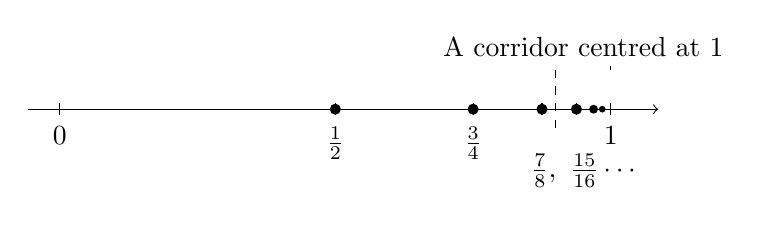
\begin{tikzpicture}[scale=1]
  \draw[->] (-0.4,0) -- (7.6,0);
  \foreach \x in {0,3.5,5.25,6.125,6.5625,7}
    \draw (\x,0.08) -- (\x,-0.08);
  \node[below] at (0,-0.1) {$0$};
  \node[below] at (3.5,-0.1) {$\frac{1}{2}$};
  \node[below] at (5.25,-0.1) {$\frac{3}{4}$};
  \node[below] at (6.65,-0.45) {$\frac{7}{8},\ \frac{15}{16}\cdots$};
  \node[below] at (7,-0.1) {$1$};
  \fill (3.5,0) circle (2pt);
  \fill (5.25,0) circle (2pt);
  \fill (6.125,0) circle (2pt);
  \fill (6.5625,0) circle (2pt);
  \fill (6.78,0) circle (1.6pt);
  \fill (6.89,0) circle (1.2pt);
  \draw[dashed] (6.3,0.5) -- (6.3,-0.25);
  \draw[dashed] (7,0.55) -- (7,0.5);
  \node[above] at (6.65,0.55) {A corridor centred at $1$};
\end{tikzpicture}
\end{center}

One common misunderstanding needs emphasis: convergence is not arrival. Every term of $\dfrac{1}{n}$ is greater than $0$, and none equals $0$, yet its limit is $0$. A limit describes a trend and destination without requiring a finish-line crossing. Conversely, some sequences have no destination: $1,-1,1,-1,\cdots$ keeps jumping between two values. Any corridor narrower than $2$, centred at either $1$ or $-1$, is left repeatedly. Such a sequence \textbf{diverges}; it has no limit.

\begin{fanli}
Consider a subtler false argument: if the distance from $a_n$ to $L$ decreases with every term, then $L$ must be the limit. Take $\dfrac{1}{n}$, or $1,\frac12,\frac13,\cdots$. Its distance from $-1$ is $1+\dfrac{1}{n}$, which really does decrease! The argument would make $-1$ its limit, yet the limit is $0$. Decreasing distance is too weak a requirement: $1+\dfrac{1}{n}$ shrinks but always exceeds $1$, so it never becomes arbitrarily small. It cannot meet every positive tolerance $d$. Thus \textbf{moving steadily closer to a target and getting arbitrarily close to it are different things}. Every word in the definition matters.
\end{fanli}

\section{The Central Theorem: Infinitely Many Shrinking Terms Can Have a Definite Sum}

With the language of limits, we can finally answer Zeno directly. First state a precise proposition.

\begin{dingli}[The Sum of an Infinite Geometric Sequence]\label{ch9:geo}
Let $a,ar,ar^2,ar^3,\cdots$ be a geometric sequence with first term $a$ and common ratio $r$, where $|r|<1$. Its first $n$ terms give the partial sum
\[
S_n=a+ar+ar^2+\cdots+ar^{n-1}.
\]
As $n$ increases without bound, $S_n$ converges and
\[
\lim_{n\to\infty}S_n=\frac{a}{1-r}.
\]
This limit is called the sum of the infinite geometric sequence, written
\[
a+ar+ar^2+\cdots=\frac{a}{1-r}.
\]
\end{dingli}

Notice the wording. The theorem does not ask us to perform infinitely many additions, an operation we cannot carry out. It says that the finite sums $S_n$ form a convergent sequence, and we \textbf{define} the infinite sum as its limit. Infinite summation is another name for a limit. This distinction unlocks Zeno's paradox.

\begin{proof}
There are two steps. First obtain a compact expression for $S_n$ using the familiar algebraic trick of shifting and subtracting. Starting from
\[
S_n=a+ar+ar^2+\cdots+ar^{n-1},
\]
multiply both sides by $r$:
\[
rS_n=ar+ar^2+\cdots+ar^{n-1}+ar^{n}.
\]
Subtract, cancelling every middle term and leaving only the ends:
\[
S_n-rS_n=a-ar^n,
\qquad\text{so}\qquad
S_n=\frac{a(1-r^n)}{1-r}.
\]
Second, apply the limit definition as $n$ grows. Rewrite this as
\[
S_n=\frac{a}{1-r}-\frac{a}{1-r}\,r^n.
\]
Since $|r|<1$, the absolute value of $r^n$ shrinks as $n$ increases. For example, with $r=0.1$, $r^n$ runs through $0.1,0.01,0.001,\cdots$. Given any positive $d$, sufficiently large $n$ makes $|r^n|$ small enough that $\left|\dfrac{a}{1-r}\right|\cdot|r^n|<d$. Thus the distance from $S_n$ to $\dfrac{a}{1-r}$ becomes arbitrarily small, so by definition
\[
\lim_{n\to\infty}S_n=\frac{a}{1-r}.
\]
Both steps use ordinary algebra and inequalities, yet together they cross infinity.
\end{proof}

The condition $|r|<1$ is essential. With $r=2$, the sum $1+2+4+8+\cdots$ grows without bound and its partial sums do not converge. With $r=-1$, the sum $1-1+1-1+\cdots$ has partial sums alternating between $1$ and $0$, again without a limit. Both diverge, so $\dfrac{a}{1-r}$ cannot be used. A theorem's conditions resemble an appliance's rated voltage: connect it incorrectly and even a beautiful formula burns out.

Pause at the proof's second step. Why trust it? Because every claim can be checked. Doubt that $r^n$ can become arbitrarily small? Take $r=\dfrac{1}{2}$. If you demand $d=10^{-9}$, I choose $n=31$, giving $2^{-31}<10^{-9}$. Demand a smaller $d$ and I supply a larger $n$. No mysticism, just an answer to every challenge.

\begin{tuilun}[Resolving Zeno's Paradox]
The time Achilles needs to catch the tortoise is the limit of the sums of the stage times:
\[
10+1+0.1+0.01+\cdots=\frac{10}{1-0.1}=\frac{100}{9}\ \text{seconds}.
\]
Infinitely many stages need not take infinitely long. Zeno's error was assuming that infinitely many positive numbers must sum to infinity. Our theorem supplies a counterexample.
\end{tuilun}

A picture offers another beautiful view. Begin with a square of area $1$, remove half, then half the remainder, and keep going. The successive areas removed are $\dfrac{1}{2},\dfrac{1}{4},\dfrac{1}{8},\dfrac{1}{16},\cdots$. You can see how these pieces fill the square:

\begin{center}
\begin{tikzpicture}[scale=5]
  \draw (0,0) rectangle (1,1);
  \draw (0.5,0) -- (0.5,1);
  \draw (0.5,0.5) -- (1,0.5);
  \draw (0.75,0) -- (0.75,0.5);
  \draw (0.75,0.25) -- (1,0.25);
  \node at (0.25,0.5) {$\frac{1}{2}$};
  \node at (0.75,0.75) {$\frac{1}{4}$};
  \node at (0.625,0.25) {$\frac{1}{8}$};
  \node at (0.875,0.375) {$\frac{1}{16}$};
  \node at (0.875,0.1) {$\cdots$};
\end{tikzpicture}
\end{center}

The picture says $\dfrac{1}{2}+\dfrac{1}{4}+\dfrac{1}{8}+\cdots=1$, matching $\dfrac{a}{1-r}$ with $a=\dfrac{1}{2}$ and $r=\dfrac{1}{2}$. This answers our third opening question too: the daily lengths removed from the stick sum to exactly $1$ chi. In the infinite limit, the total removed is one whole stick, with no tiny remnant. Saying that half still remains after every day describes a process that never finishes; saying that the total is exactly $1$ describes its limit. These statements concern different objects and do not conflict. Confusing process with limit is the heart of Zeno's mistake.

\section{Another Perspective: Does the Number Line Have Holes?}

So far we have asked what a limit equals. Now ask something deeper: must it exist, and what kind of number is it?

Consider
\[
1,\ 1.4,\ 1.41,\ 1.414,\ 1.4142,\ \cdots
\]
Every term is a terminating decimal and therefore rational. The terms crowd together: beyond some point, any two can be made arbitrarily close, since their shared initial decimal digits grow longer. Intuitively they should crowd toward a point on the line. We know its length, the diagonal of a square of side $1$, is $\sqrt{2}$, and $\sqrt{2}$ is not rational. If only rational numbers were allowed, the sequence would try desperately to converge with no destination available: its limit is outside the city.

It is like a lift rising steadily yet never reaching a floor, because the building lacks the required floor. The rational number line is full of such holes: mark off a diagonal with a compass, and its endpoint may fall into one.

\begin{shuyu}{Completeness of the Real Numbers}
\textbf{Intuition}: the real number line has no holes. Every sequence whose terms crowd arbitrarily closely together, later called a Cauchy sequence, has a real limit.\\
\textbf{Formal definition}: the real numbers satisfy the completeness axiom: every Cauchy sequence converges to a real number; equivalently, every set of real numbers bounded above has a least upper bound.\\
\textbf{Example}: $\sqrt{2}$ is the limit of $1,1.4,1.41,\cdots$. We need not know $\sqrt{2}$ first and then find a sequence; such a sequence can instead define $\sqrt{2}$.
\end{shuyu}

Completeness is an axiom, a property we require of the reals rather than prove here. Think of it as a building promise: whenever a sequence ought to have a limit, the corresponding point is guaranteed to be on the line. This promise supports limit theory and the entire structure of calculus.

Completeness has a simpler-looking form worth examining. Imagine a balloon growing toward a ceiling: it grows at every stage but never passes the ceiling. Intuition says it must approach some definite height. In sequence language, \textbf{a sequence whose terms never decrease and are all bounded above by one fixed number must converge}. This is the monotone convergence principle, another expression of the number line having no holes, like the Cauchy criterion. Experiment 3's sequence $\left(1+\dfrac{1}{n}\right)^n$ relies on it: it can be proved increasing and always less than $3$, so its limit exists. Mathematicians proved existence before naming the limit $e$. Remember that order: existence first, name afterward.

Now return to the second opening question: does $0.999\cdots$ equal $1$? Apply Theorem \ref{ch9:geo}. The decimal $0.999\cdots$ means the infinite sum
\[
\frac{9}{10}+\frac{9}{100}+\frac{9}{1000}+\cdots,
\]
with first term $a=\dfrac{9}{10}$ and common ratio $r=\dfrac{1}{10}$, so
\[
0.999\cdots=\frac{\frac{9}{10}}{1-\frac{1}{10}}=\frac{\frac{9}{10}}{\frac{9}{10}}=1.
\]
It is exactly $1$, with no shortfall. If this feels uncomfortable, you may be picturing $0.999\cdots$ as a number still climbing toward $1$ without reaching it. But it denotes the limit of an infinite sum, whose value is $1$, rather than the process. Thus $1$ and $0.999\cdots$ are two representations of the same real number, like $\dfrac{1}{2}$ and $\dfrac{2}{4}$ for the same fraction. Every terminating decimal has such a twin representation; for example, $0.5=0.4999\cdots$.

\begin{lianjie}
Limits belong beyond pure mathematics. Ideal gases, smooth inclines, and instantaneous velocities in science are products of limits: real gas molecules have size, and an ideal gas lets that size tend to $0$; real inclines have friction, and a smooth one lets friction tend to $0$. Engineers simulating weather or designing chips use the reverse operation, dividing continuous change into finitely many computational steps, with more steps approaching reality more closely. Every weather forecast on your phone comes from finite steps approximating the infinite. Our limits underpin next chapter's derivative: the limit of average rates of change as a time interval tends to $0$.
\end{lianjie}

\begin{toolbox}
This chapter's new tools:
\begin{itemize}
  \item \textbf{Sequences}: divide an infinite process into stages and study the ordered list of results.
  \item \textbf{The limit definition, or corridor game}: for every positive $d$, there exists $N$ such that $n>N$ implies $|a_n-L|<d$. Infinite approach becomes a checkable inequality.
  \item \textbf{Infinite geometric sums}: if $|r|<1$, then $a+ar+ar^2+\cdots=\dfrac{a}{1-r}$. An infinite sum is a limit of partial sums, not an addition performed infinitely many times.
  \item \textbf{Completeness}: the real line has no holes, so sequences that should converge have destinations.
\end{itemize}
\end{toolbox}

\section{Mathematical Experiments}

\begin{shiyan}
\textbf{Experiment 1: Adding Toward an Infinite Sum.} Use a calculator to compute
\[
\frac{1}{2},\quad \frac{1}{2}+\frac{1}{4},\quad \frac{1}{2}+\frac{1}{4}+\frac{1}{8},\quad \cdots
\]
Record each result, continuing at least through $\dfrac{1}{2^{10}}=\dfrac{1}{1024}$. You obtain $0.5,0.75,0.875,0.9375,\cdots$. Each term added halves the distance to $1$. After how many terms is the distance to $1$ less than $0.001$? In the corridor game, which $N$ corresponds to your demand $d=0.001$?

\textbf{Experiment 2: Building an Approximation Road to $\sqrt{2}$.} Use only arithmetic, without the square-root key. Start with $[1,2]$ and test the midpoint $1.5$. Since $1.5^2=2.25>2$, $\sqrt{2}$ lies in $[1,1.5]$. Test the next midpoint, $1.25$, comparing its square with $2$ to choose the left or right half. Each step halves the interval. Perform $8$ steps and record the endpoints; you will obtain $\sqrt{2}\approx 1.414$. What does this nested-interval process share with the decimal approximations $1,1.4,1.41,\cdots$? If the number line had holes, would the experiment still guarantee a number trapped inside?

\textbf{Experiment 3 (Optional): A Magical Number.} Calculate $\left(1+\dfrac{1}{n}\right)^n$. For $n=1$ it is $2$; for $n=10$, about $2.594$; for $n=100$, about $2.705$; and for $n=1000$, about $2.717$. It seems to converge to a mysterious number beginning $2.718$. Record the observation; the exercises return to it.
\end{shiyan}

\section*{Questions to Think About}

\textbf{Observation}
\begin{sikao}
  \item Examine $\dfrac{1}{2},\dfrac{2}{3},\dfrac{3}{4},\dfrac{4}{5},\cdots$, whose $n$th term is $\dfrac{n}{n+1}$. Calculate early terms to guess the limit, then find the distance between the $n$th term and that limit. \textbf{Hint}: rewrite $\dfrac{n}{n+1}$ as $1-\dfrac{1}{n+1}$.
  \item Use this chapter's theorem to express $0.333\cdots$ and $0.121212\cdots$ as fractions. What is the common ratio for the second decimal? \textbf{Hint}: $0.121212\cdots$ repeats every two digits, so it is a geometric sum with first term $\dfrac{12}{100}$ and ratio $\dfrac{1}{100}$.
\end{sikao}

\textbf{Proof}
\begin{sikao}
  \item Use the corridor game to prove rigorously that $\dfrac{1}{n}$ converges to $0$. For any positive $d$, give an explicit $N$, allowed to depend on $d$, and explain why $n>N$ implies $\left|\dfrac{1}{n}-0\right|<d$. \textbf{Hint}: all you need is $\dfrac{1}{n}<d$. Take reciprocals to see how large $n$ must be.
  \item Prove that a sequence cannot converge to two different numbers $L$ and $M$. \textbf{Hint}: let their distance be $h>0$. Choose $d=\dfrac{h}{2}$ and draw corridors centred at $L$ and $M$. They do not overlap. What contradiction arises if the sequence must eventually stay in both?
\end{sikao}

\textbf{Challenge}
\begin{sikao}
  \item Experiment 3's sequence $\left(1+\dfrac{1}{n}\right)^n$ appears to converge. Investigate or think about its limit, the natural constant $e$, approximately $2.71828$. Every term is rational, but $e$ is irrational. Why is this unsurprising in light of completeness? \textbf{Hint}: recall $\sqrt{2}$. The types of the individual terms and the type of their limit are separate questions.
  \item Zeno's arrow paradox says that a flying arrow occupies a definite position at each instant, so it is stationary at each instant and therefore never moves. Identify the gap using this chapter's language. \textbf{Hint}: does the leap from definite position to no motion again confuse a process with a limit? How should velocity at an instant be defined? That is next chapter's problem.
\end{sikao}

\begin{pandeng}
Further climbing brings these sights: replace $d$ by the Greek letter $\varepsilon$ and justify $N$ rigorously to obtain the $\varepsilon$--$N$ language of university analysis. The precise statement that terms crowding together have a limit is the Cauchy convergence criterion, equivalent to monotone bounded convergence as a form of completeness. General infinite series extend geometric sums, and deciding convergence or divergence begins series theory. The limit $e$ of $\left(1+\frac{1}{n}\right)^n$ returns in logarithms, compound interest, and differential equations. Competition methods using upper and lower bounds, including the squeeze theorem---both sides approach $L$, leaving the middle no escape---are variations on the corridor game.
\end{pandeng}

\section*{The Door to the Next Chapter}

We have tamed the accumulation of infinitely many quantities, but Zeno's arrow still hangs in the air with a trickier question: what is velocity at a single instant?

A car's dashboard says $60$ kilometres per hour. Where does that number come from? Speed is distance divided by time, but in one instant the distance is $0$ and the time is $0$. What is $\dfrac{0}{0}$? It gives no answer. Intuition has failed again.

You have already glimpsed the way out: replace the instant with a short interval beginning there. Calculate average speeds over $1$ second, $0.1$ seconds, $0.01$ seconds, and so on. If these averages form a convergent sequence, its limit deserves the name instantaneous velocity. Likewise, a curve's tangent slope is the limit of secant slopes as the two points approach each other.

The limit of average rates of change is the derivative. Next chapter, we bring the corridor game into the world of functions to measure change itself precisely.
